\begin{figure*}[htbp]
    \centering
    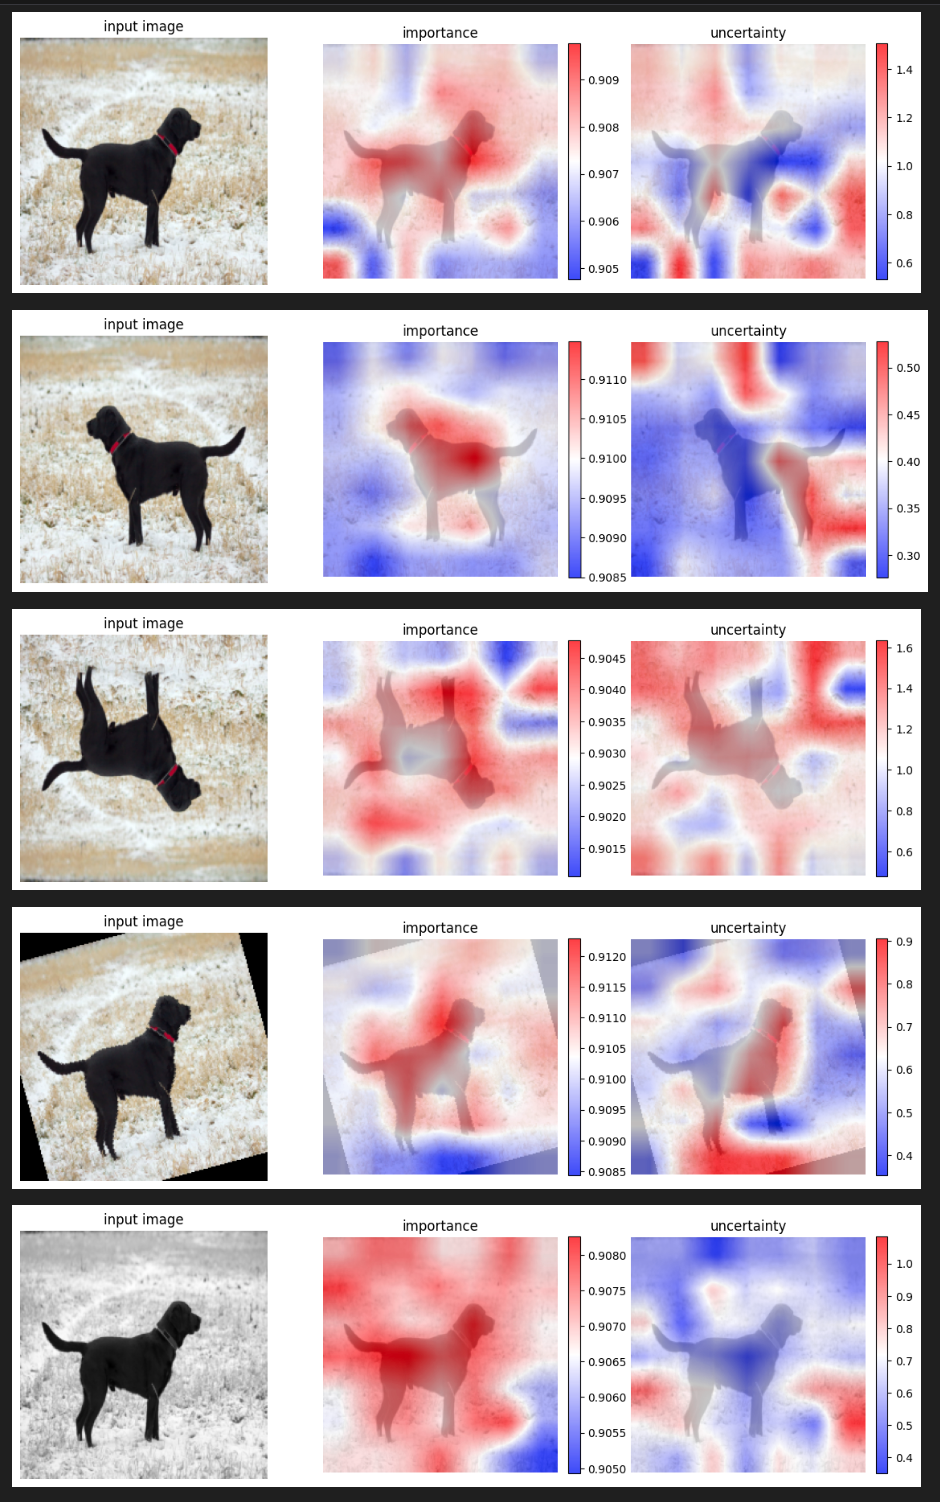
\includegraphics[width=\textwidth, height=0.75\textheight, keepaspectratio]{images/swav_relax.png}
    \caption{RELAX visualizations for the SwAV model across various augmentations: horizontal flip, vertical flip, 15° rotation, and grayscale. Importance maps remain focused on the object (dog), and uncertainty is relatively low, showcasing SwAV's strong spatial invariance and robust attention.}
    \label{fig:swav_relax}
\end{figure*}

\begin{figure*}[htbp]
    \centering
    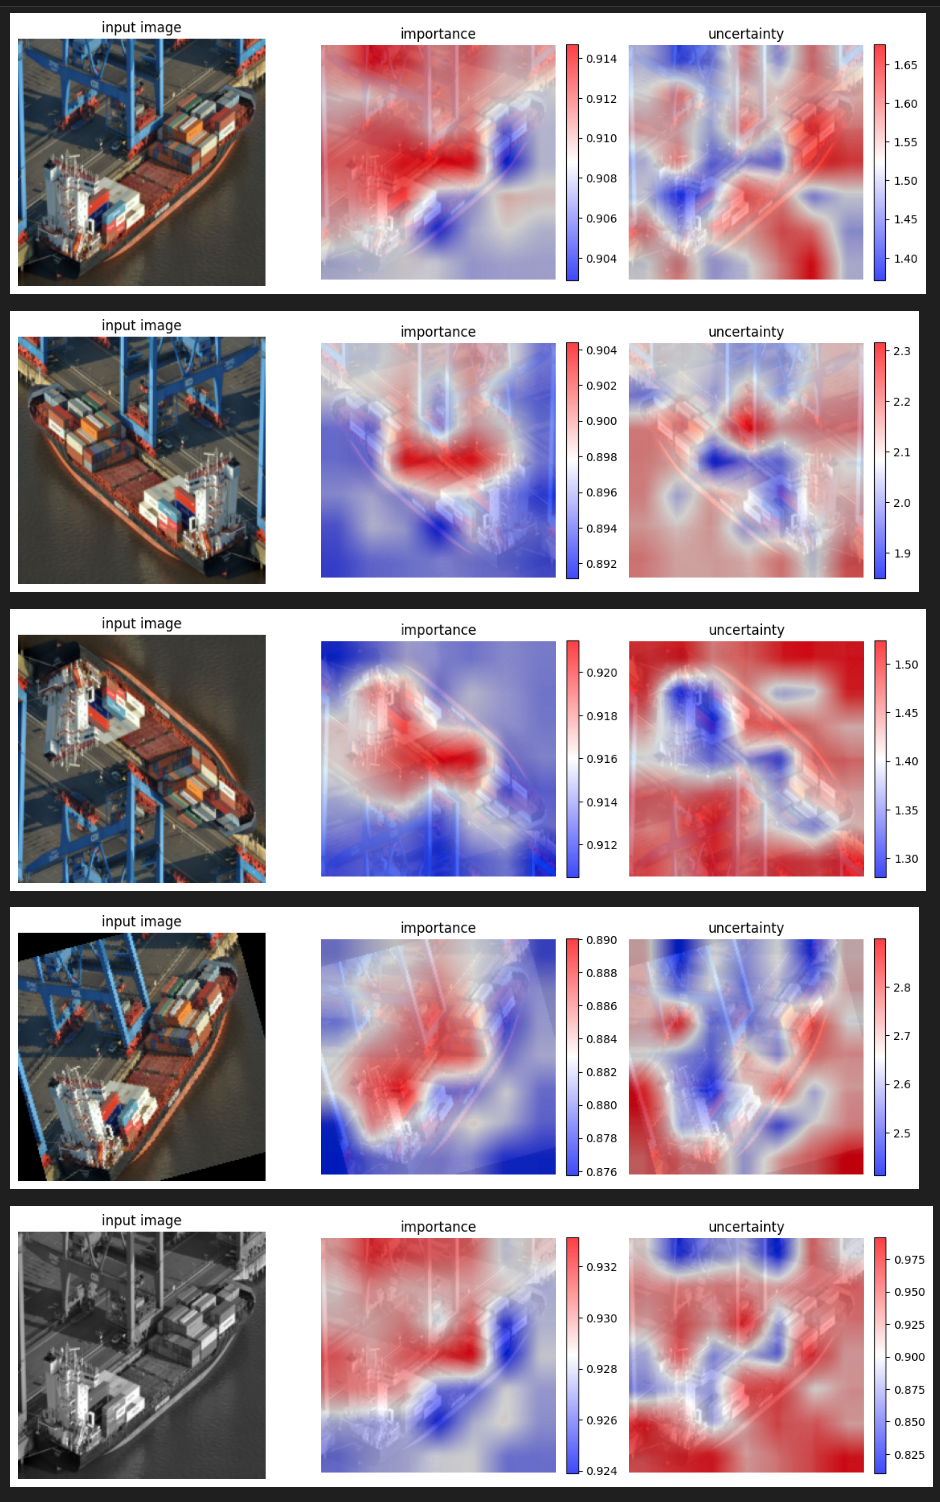
\includegraphics[width=\textwidth, height=0.75\textheight, keepaspectratio]{images/moco_relax.png}
    \caption{RELAX visualizations for the MoCo model under similar augmentations. The model exhibits higher uncertainty and shifting importance regions, particularly under strong geometric changes, suggesting comparatively lower invariance and stability.}
    \label{fig:moco_relax}
\end{figure*}

\begin{figure*}[htbp]
    \centering
    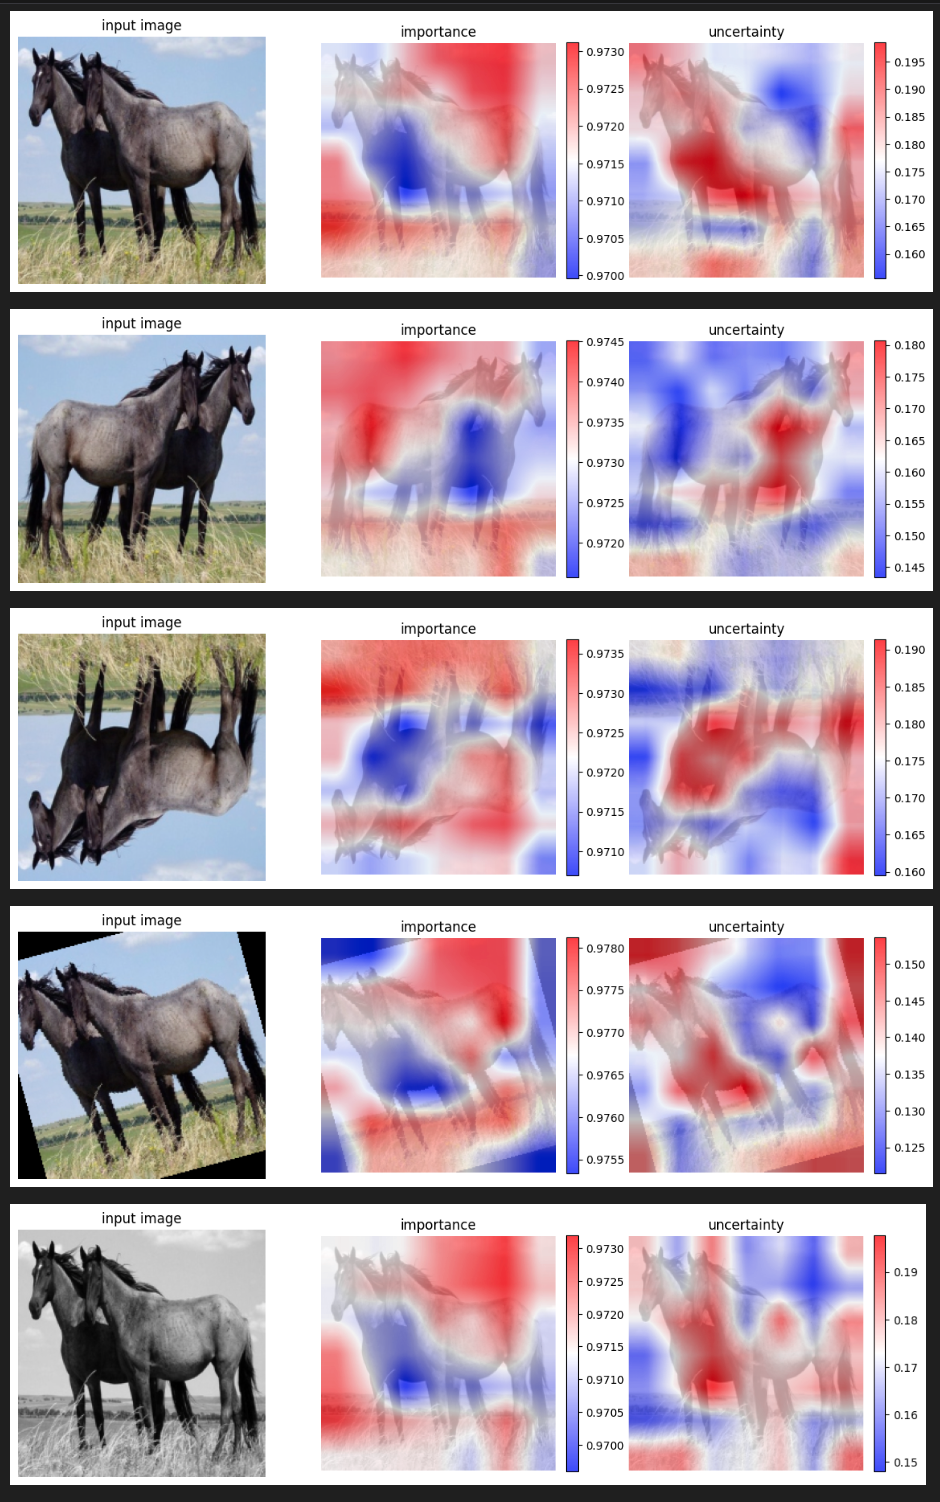
\includegraphics[width=\textwidth, height=0.75\textheight, keepaspectratio]{images/simclr_relax.png}
    \caption{RELAX visualizations for SimCLR (trained from scratch on CIFAR-10). The importance regions are generally focused on the objects (horses), but there is moderate spatial drift and variable uncertainty across augmentations, reflecting a balance between sensitivity and consistency.}
    \label{fig:simclr_relax}
\end{figure*}

\begin{figure*}[htbp]
    \centering
    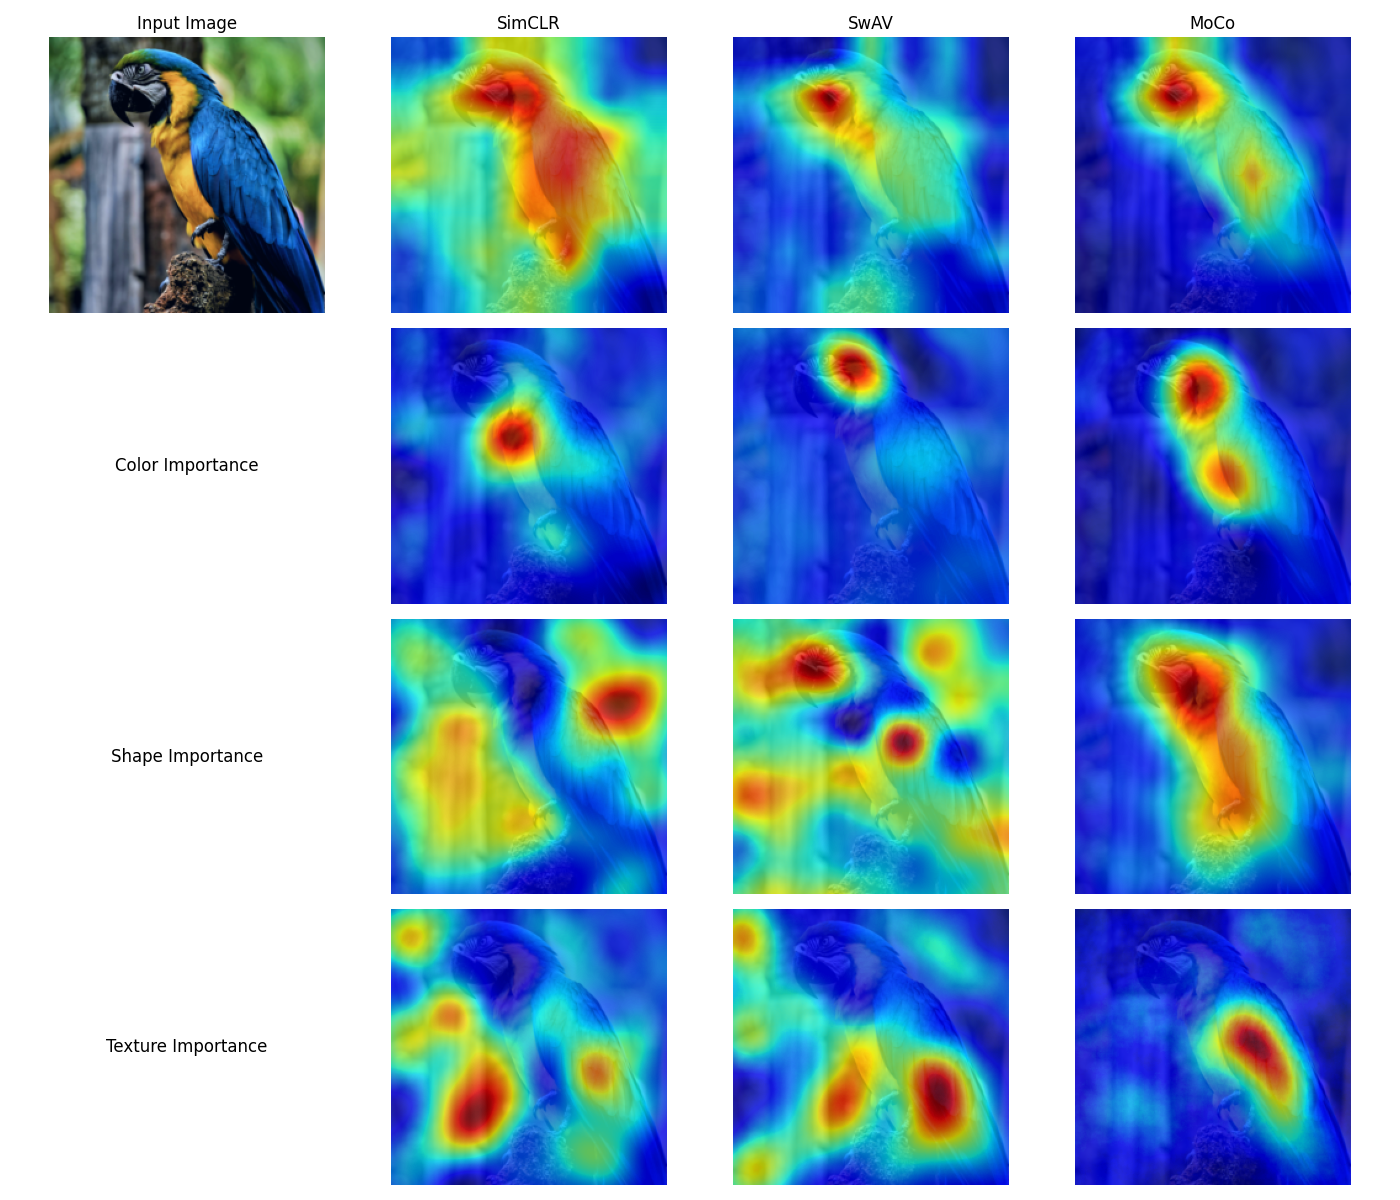
\includegraphics[width=\textwidth, height=0.75\textheight, keepaspectratio]{images/Perceptual Components Importance Using RELAX.png}
    \caption{Perceptual importance maps showing the contribution of color, shape, and texture features across three models—SimCLR, SwAV, and MoCo—using the RELAX explanation method.}
    \label{fig:relax_perceptual_maps}
\end{figure*}

\begin{figure*}[htbp]
    \centering
    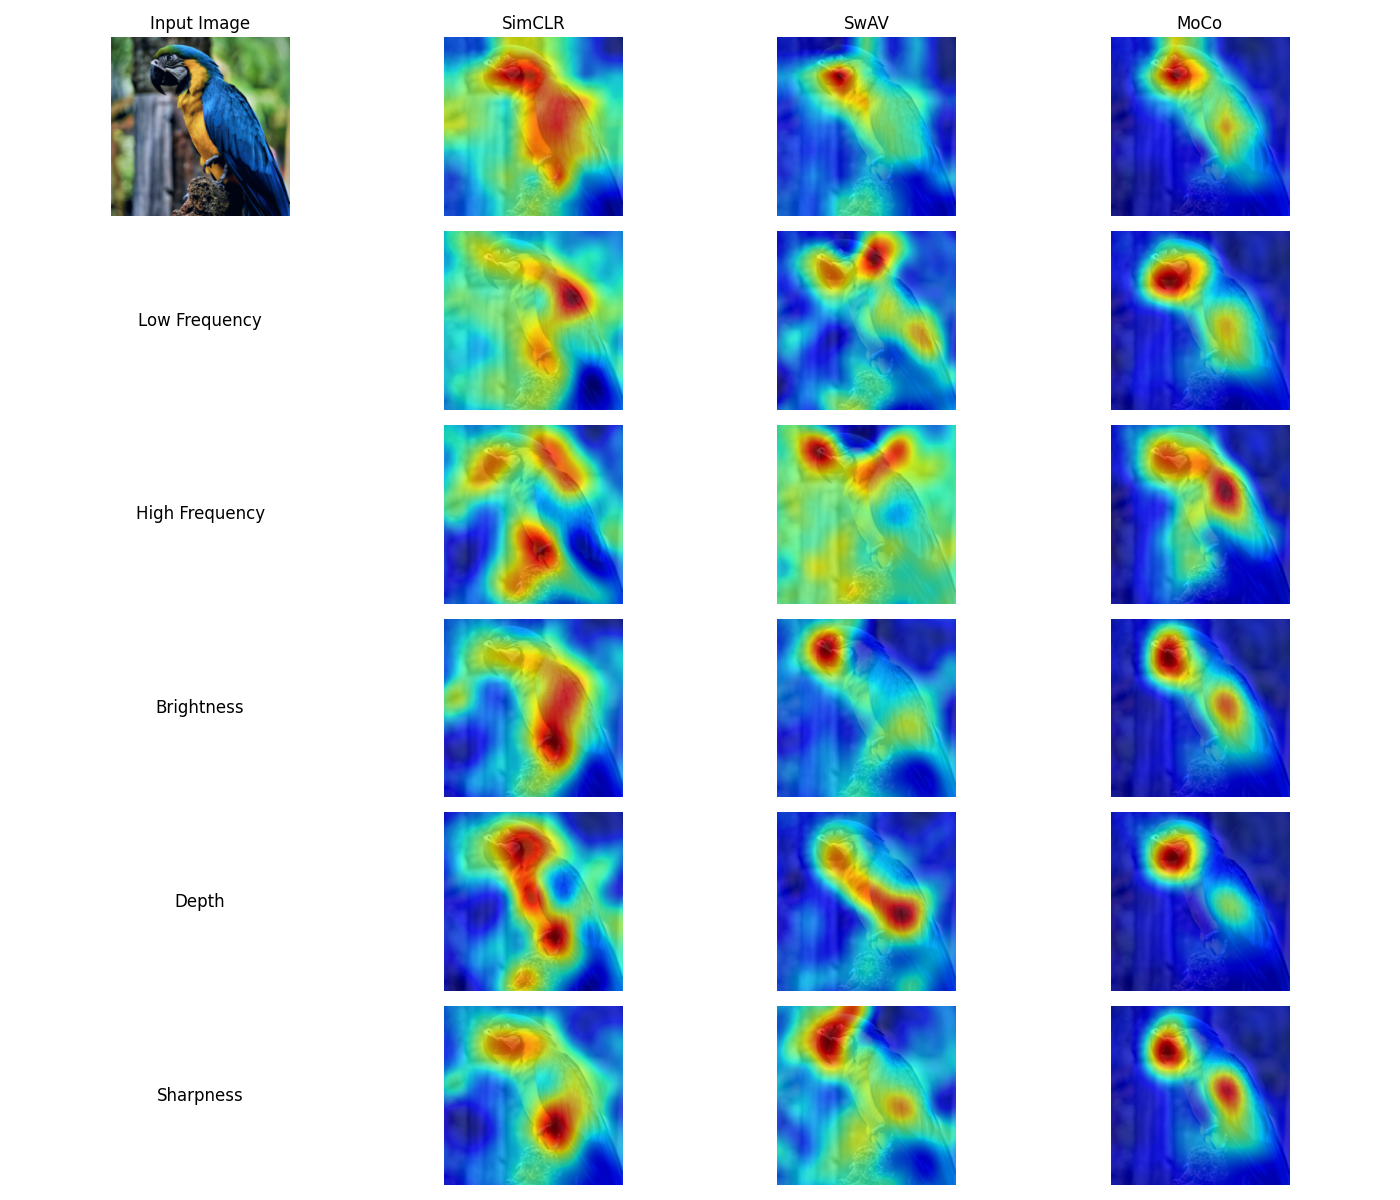
\includegraphics[width=\textwidth, height=0.75\textheight, keepaspectratio]{images/Perceptual Components Importance Using RELAX Extended.png}
    \caption{Extended perceptual component attribution maps including low-frequency, high-frequency, brightness, depth, and sharpness, comparing the same three models. These help identify additional cues the models may implicitly rely on.}
    \label{fig:relax_extended_components}
\end{figure*}